\begin{figure}[tb]
\centering
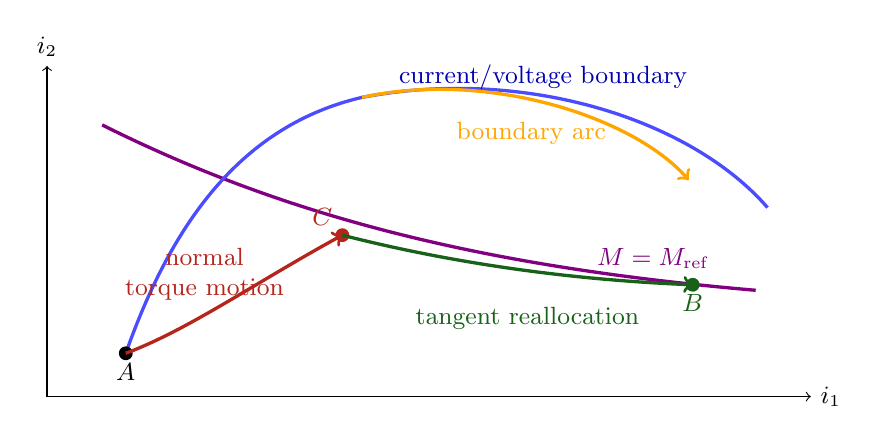
\begin{tikzpicture}[font=\small,x=1cm,y=1cm]
 \draw[->] (0,0)--(9.7,0) node[right] {$i_1$};
 \draw[->] (0,0)--(0,4.2) node[above] {$i_2$};
 \draw[Purple,very thick] (.7,3.45)..controls(3.0,2.3)and(5.5,1.65)..(9.0,1.35);
 \node[Purple] at (7.7,1.75) {$M=M_{\rm ref}$};
 \draw[blue!70,very thick] (1.0,.55)..controls(1.6,2.25)and(2.5,3.45)..(4.0,3.8)
   ..controls(6.1,4.2)and(8.2,3.5)..(9.15,2.4);
 \node[blue!70!black] at (6.3,4.05) {current/voltage boundary};
 \fill (1.0,.55) circle (2.5pt) node[below] {$A$};
 \fill[BrickRed] (3.75,2.05) circle (2.5pt) node[above left] {$C$};
 \fill[ForestGreen!70!black] (8.2,1.42) circle (2.5pt) node[below] {$B$};
 \draw[BrickRed,very thick,->] (1.0,.55)..controls(1.8,.85)and(2.65,1.45)..(3.75,2.05);
 \draw[ForestGreen!70!black,very thick,->] (3.75,2.05)..controls(5.2,1.68)and(6.7,1.48)..(8.2,1.42);
 \node[BrickRed,align=center] at (2.0,1.55) {normal\\torque motion};
 \node[ForestGreen!70!black] at (6.1,1.0) {tangent reallocation};
 \draw[Orange,very thick,->] (4.0,3.8)..controls(5.6,4.15)and(7.45,3.55)..(8.15,2.75);
 \node[Orange] at (6.15,3.35) {boundary arc};
\end{tikzpicture}
\caption{Two geometric structures that may coexist: hierarchical
torque acquisition followed by tangent reallocation, and a minimum-time
boundary arc that uses an active physical constraint as a road.}
\label{fig:two-stage-boundary}
\end{figure}

